\section{Mode 1 - Static mode}
\subsection {Mode description}
The first mode allows user to select and write letters. In the english alphabet there are 26 letters, so to be able to use all of them at least 26 gestures had to be specified and implemented. The aim was to produce a program which is as simple as possible, because a too complicated set of movements and signs wouldn't have been user-friendly and straightforward to use. The scheme is shown in the Figure \ref{fig:letters}.

\begin{figure}[H]
	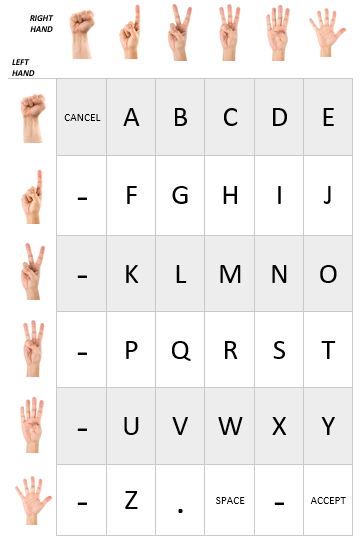
\includegraphics{static_gestures}
	\centering
	\caption{Letter selection - set of gestures}
	\label{fig:letters}
\end{figure}

Every letter and command has its own and unique command. \textbf{Differentation is done by counting the number of extended fingers in each hands}. This makes the set gesture straighfoward to learn. For instance, when only one finger in the left hand is extended and at the same time, the right hand is fully open, the letter "J" should be detected.\\

However, sometimes the wrong letter can be selected. To avoid writing unwanted letter on the paper, two additional gestures were added :
\begin{itemize}
	\item the command "Accept" to validate the selected letter send the writing command to the robot;
	\item the command "Cancel" to restart the selection.
\end{itemize}

We also wanted to be able to write full sentences. Thus, we decided to implement gesture to draw the dot and the space characters. It is easy to see in the Figure \ref{fig:letters} that there are 6 more possible gestures that are not used. Also the set of gestures could be easily extended.

\subsection{Letters library}

Additionally to the sign alphabet, a library of letter has been created. This library is, in fact, a set of movements which have to be done by the robot in order to write each of the letters. Each set of movements includes moving in all of the three space dimensions (x, y, z). Letters library is built in such way that every letter is written in a rectangle of sides length of b and a, and left down corner coordinates of (c, d). After finishing all of the movements for a letter, the last move is used to obtain new starting position for the next letter, so the point of coordinate (c, d) is updated after every new letter. It allows robot to write letters next to each other, which makes writing words or sentences possible. Starting point (c,d) as well as z1, z2 (z1 being the position on the z axis when the marker is not touching the surface and z2 being the writing position) and sides lengths of a and b might be specified by user at the beginning of this program, which makes it more universal and multifunctional.\\

\begin{figure}[H]
	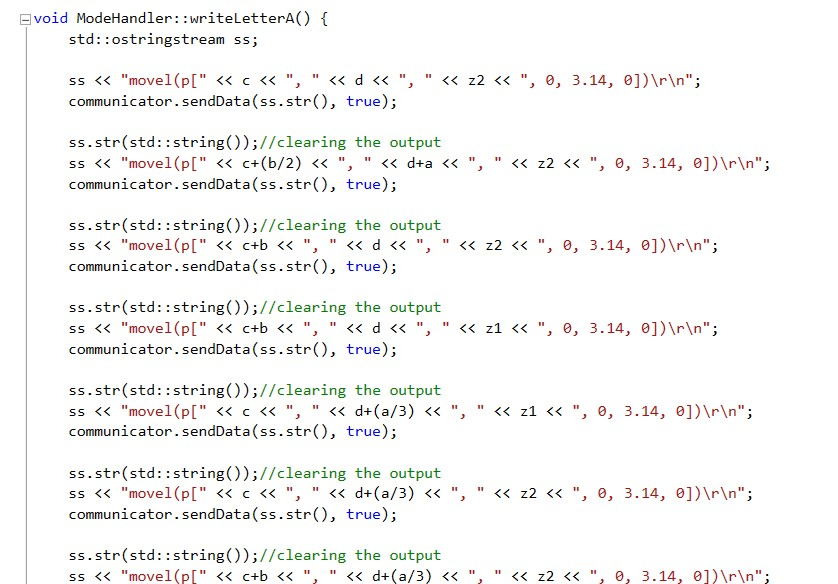
\includegraphics[scale=0.8]{Aletter}
	\centering
	\caption{Example code from letter library}
	\label{fig:Aletter}
\end{figure}

Functions \textit{writeLetter} are constructed in such a way that the whole command is send to the robot controller, in this case it is the command \textit{movel(p[x, y, z, 0, 3.14, 0]}. This kind of communication was chosen because of the possibilities of changing the coordinates of the starting point (c, d), which is a crucial part for the project main idea and it was not possible or much more complicated to use other methods of working with the robot. What is more, the function \textit{movel} was chosen because of its functionality – this function makes robot move in straight line, without changing the position of the robot’s head (which is the main difference with the other command \textit{movej} which reaches the target position in the shortest possible way, which is not necessarily the straight line). After sending the command, a delay is set before sending the next command in order to allow the robot to finish the first task. If there was no delay, the robot’s controller, after receiving a pack of commands, would perform only the last one, which means that the idea of using delay is crucial for program operation. An example function for writing letter is given in the Figure \ref{fig:Aletter}. \\

The result of this set of movement is given in Figure\ref{fig:letter}, showing the letter A written by the robot’s arm after the Leap Motion recognised, first the gesture responsible for enabling mode 1, then the gesture responsible for letter A and, finally, the gesture of acceptance. Inaccuracies visible in the Figure\ref{fig:letter} result from inappropriate marker placement and not because of the program. Those could be improved in case of other program tests. \\

\begin{figure}[H]
	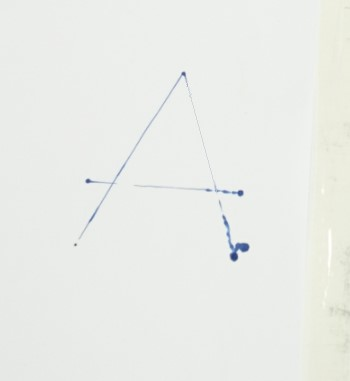
\includegraphics{letter}
	\centering
	\caption{Example code from letter library}
	\label{fig:letter}
\end{figure}

Prepared letters library is only one example of possible library which could be created for this kind of program. Since designed gestures are meant to be simple and intuitive for any user, they can be used with other libraries like handwritten letters, small letters, numbers and any non-Latin alphabet etc., which makes this program more universal and user-friendly. Set of gestures are not too difficult to obtain, but need time to be prepared correctly. Its main advantage is the fact that one they are written, there is no need to worry about robot’s movements after launching the program. To make it easier for user, in case of future work, additional application could be proposed, which would automatically prepare set of gestures and save them in program’s memory.
